
\documentclass[12pt]{article}

% Layout.
\usepackage[top=1in, bottom=0.75in, left=1in, right=1in, headheight=1in, headsep=6pt]{geometry}

% Fonts.
\usepackage{mathptmx}
\usepackage[scaled=0.86]{helvet}
\renewcommand{\emph}[1]{\textsf{\textbf{#1}}}

% TiKZ.
\usepackage{tikz, pgfplots}
\usetikzlibrary{calc}
\pgfplotsset{compat = newest}
 
\pgfplotsset{my style/.append style={axis x line=middle, axis y line=
middle, xlabel={$x$}, ylabel={$y$}, axis equal }}

% Misc packages.
\usepackage{amsmath,amssymb,latexsym}
\usepackage{graphicx}
\usepackage{array}
\usepackage{xcolor}
\usepackage{multicol}

% Commands to set various header/footer components.
\makeatletter
\def\doctitle#1{\gdef\@doctitle{#1}}
\doctitle{Use {\tt\textbackslash doctitle\{MY LABEL\}}.}
\def\docdate#1{\gdef\@docdate{#1}}
\docdate{Use {\tt\textbackslash docdate\{MY DATE\}}.}
\def\doccourse#1{\gdef\@doccourse{#1}}
\let\@doccourse\@empty
\def\docscoring#1{\gdef\@docscoring{#1}}
\let\@docscoring\@empty
\def\docversion#1{\gdef\@docversion{#1}}
\let\@docversion\@empty
\makeatother

% Headers and footers layout.
\makeatletter
\usepackage{fancyhdr}
\pagestyle{fancy}
\fancyhf{} % Clears all headers/footers.
\lhead{\baselineskip 30pt
%\emph{\@doctitle\hfill\@docdate}
\emph{\@docdate\hfill\@doctitle}
\ifnum \value{page} > 1\relax\else\\
\emph{Name: \rule{3.5in}{1pt}\hfill \@docscoring}\fi}
\rfoot{\emph{\@docversion}}
\lfoot{\emph{\@doccourse}}
\cfoot{\emph{\thepage}}
\renewcommand{\headrulewidth}{0pt}%
\makeatother

% Paragraph spacing
\parindent 0pt
\parskip 6pt plus 1pt

% A problem is a section-like command. Use \problem{5} to
% start a problem worth 5 points.
\newcounter{probcount}
\newcounter{subprobcount}
\setcounter{probcount}{0}
\newcommand{\problem}[1]{%
\par
\addvspace{4pt}%
\setcounter{subprobcount}{0}%
\stepcounter{probcount}%
\makebox[0pt][r]{\emph{\arabic{probcount}.}\hskip1ex}\emph{[#1 points]}\hskip1ex}
\newcommand{\thesubproblem}{\emph{\alph{subprobcount}.}}

% Subproblems are an enumerate-like environment with a consistent
% numbering scheme. 
% Use \begin{subproblems}\item...\item...\end{subproblems}
\newenvironment{subproblems}{%
\begin{enumerate}%
\setcounter{enumi}{\value{subprobcount}}%
\renewcommand{\theenumi}{\emph{\alph{enumi}}}}%
{\setcounter{subprobcount}{\value{enumi}}\end{enumerate}}

% Blanks for answers in normal and math mode.
\newcommand{\blank}[1]{\rule{#1}{0.75pt}}
\newcommand{\mblank}[1]{\underline{\hspace{#1}}}
\def\emptybox(#1,#2){\framebox{\parbox[c][#2]{#1}{\rule{0pt}{0pt}}}}

% Misc.
\renewcommand{\d}{\displaystyle}
\newcommand{\ds}{\displaystyle}
\def\bc{\begin{center}}
\def\ec{\end{center}}
\def\be{\begin{enumerate}}
\def\ee{\end{enumerate}}


\doctitle{Math 251: Quiz 2}
\docdate{January 25, 2024}
\doccourse{UAF Calculus I}
\docversion{v-1}
\docscoring{\blank{0.8in} / 25}
\begin{document}
%\textbf{Please circle your instructor's name:} \hfill Leah Berman  \hfill   Jill Faudree\\

There are 25 points possible on this quiz. No aids (book, calculator, etc.)
are permitted.  {\bf Show all work for full credit.}

\problem{11} Let $P(2,2)$ be a point on the graph of $f(x)=\displaystyle{\frac{6x-6}{x+1}}.$
\begin{subproblems}
\item Find the slope of the secant line passing through $P$ and the point $Q(1,f(1)).$ 
\vfill

\item Find the slope of the secant line passing through $P$ and the point $Q(3,f(3)).$

\vfill

\item The table below lists the slope of the secant line passing through the point $P$ and the point $Q(x, f(x))$ for several values of $x.$ \\

\begin{tabular}{l || c|c|c|c|c|c}
x&1.9&1.99&1.999&2.001&2.01&2.1\\
\hline
f(x)&1.8621&1.9866&1.9987& 2.0013&2.0133 &2.1290 \\
\hline
$m_{sec}$&1.3793 &1.3378&1.3338&1.3328&1.3289&1.2903\\
\end{tabular}

\vskip 0.5cm
Use the information in the table to estimate the slope of the tangent line to $f(x)$ at the point $P(2,2).$
\vfill

\item Use the slope from part (c) above to write an equation of the tangent line at point $P.$

\vfill

\item Below is a sketch of the graph of $f(x)=\frac{6x-6}{x+1}.$ Sketch the tangent line to the graph at the point $P.$

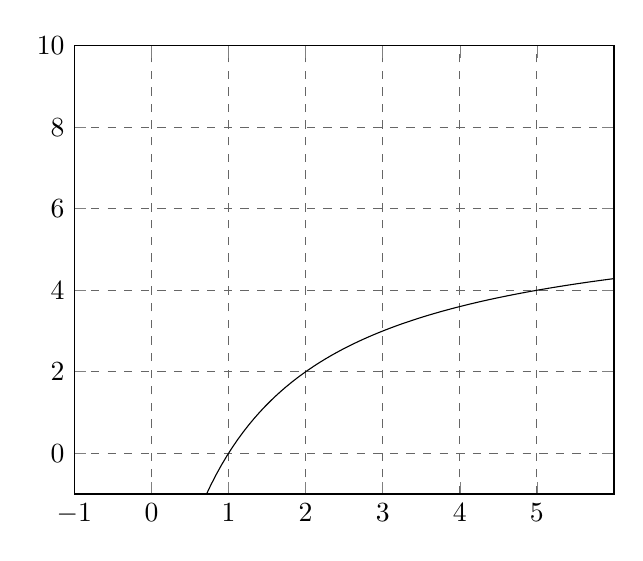
\begin{tikzpicture}
 \begin{axis}[
    xmin = -1, xmax = 6,
    ymin = -1, ymax = 10, xtick={-1,0,...,5}, ytick={-2,0,...,10},
    grid=both, grid style={ thin, black!60, dashed}]
    \addplot[samples=100,
        domain = -1:6,
    ] {(6*x-6)/(x+1)};
    %\addplot[thick,->] coordinates {(-1,0) (6,0)};
\end{axis}
\end{tikzpicture}

\end{subproblems}
\newpage

\problem{9}
Use the graph of the function of $f(x)$ to answer the following questions. Give the most complete answer; if the limit is infinite, indicate that with $\infty$ or $-\infty.$ If a value does not exist, write DNE.\\
\begin{center}
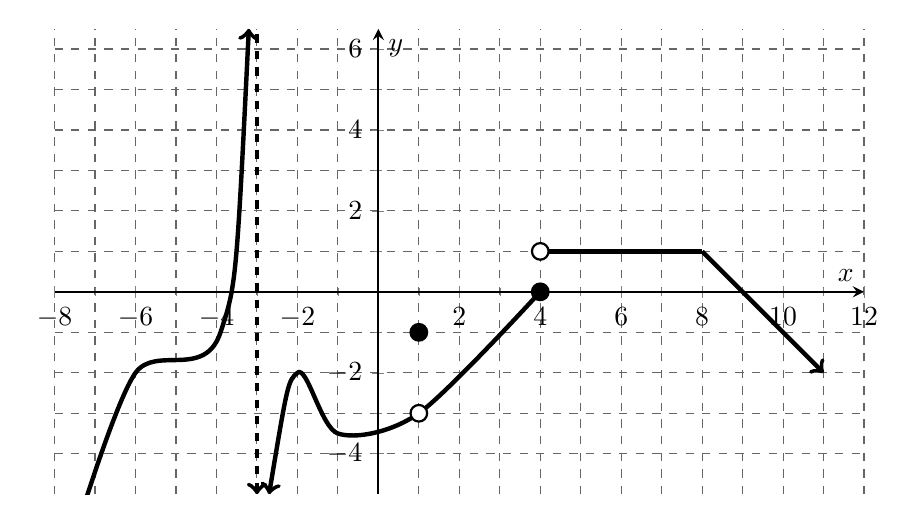
\begin{tikzpicture}
\begin{axis}[scale=1.5, thick, my style, xtick={-8,-6,...,12}, ytick={-4,-2,...,6},
xmin=-8, xmax=12, ymin=-5, ymax=6.5, minor y tick num=1,
        minor x tick num=1, mark size=3.0pt, grid=both, grid style={ thin, black!60, dashed}, axis equal image]
% %%asymptote
\addplot[dashed,<->, ultra thick] coordinates {(-3,-5) (-3,12)};       
%%points solid
\addplot[mark=*,only marks] coordinates {(4,0)(1,-1)};
%%points open
\addplot[mark=*,fill=white,only marks] coordinates {(4,1)(1,-3)};
%%Curves
\addplot[ultra thick, smooth,<->] coordinates {(-3.2,6.5) (-3.9,-1) (-6, -2) (-7.5,-6)};
\addplot[ultra thick, smooth,<-] coordinates {(-2.7,-5) (-2,-2) (-1,-3.5) (1,-3) (4,0)};
\addplot[ultra thick, smooth] coordinates {(4,1) (8,1)};
\addplot[ultra thick, smooth,->] coordinates {(8,1) (11,-2)};       

\end{axis}
\end{tikzpicture}
\end{center}

\begin{subproblems}
\begin{multicols}{3}
\item $f(-2)=\mblank{.5in}$
\item $f(1)=\mblank{.5in}$
\item $f(4)=\mblank{.5in}$
%\item $f(5)=\mblank{.5in}$
\end{multicols}
\vspace{0.1in}
\begin{multicols}{3}
\item $\d{\lim_{x \to\; -3} f(x)=\mblank{.5in}}$
\item $\d{\lim_{x \to\; -2} f(x)=\mblank{.5in}}$
\item $\d{\lim_{x \to\; 1} f(x)=\mblank{.5in}}$
\end{multicols}
\begin{multicols}{3}
\item $\d{\lim_{x \to\; 4^+} f(x)=\mblank{.5in}}$
\item $\d{\lim_{x \to 4^-} f(x)=\mblank{.5in}}$
\item $\d \lim_{x\to\; 4}f(x)=\mblank{.5in}$
\end{multicols}
\end{subproblems}

\problem{5} On the axes below, sketch a graph satisfying \emph{all} of the properties listed below.\\

\begin{tabular}{ccccc}
$\displaystyle{\lim_{x \to1^-} f(x) =2},$&$\displaystyle{\lim_{x \to1^+} f(x) =3,}$&$f(1)=5$,&
$\displaystyle{\lim_{x \to4} f(x) =5},$&$f(4)=0$\\
\end{tabular}

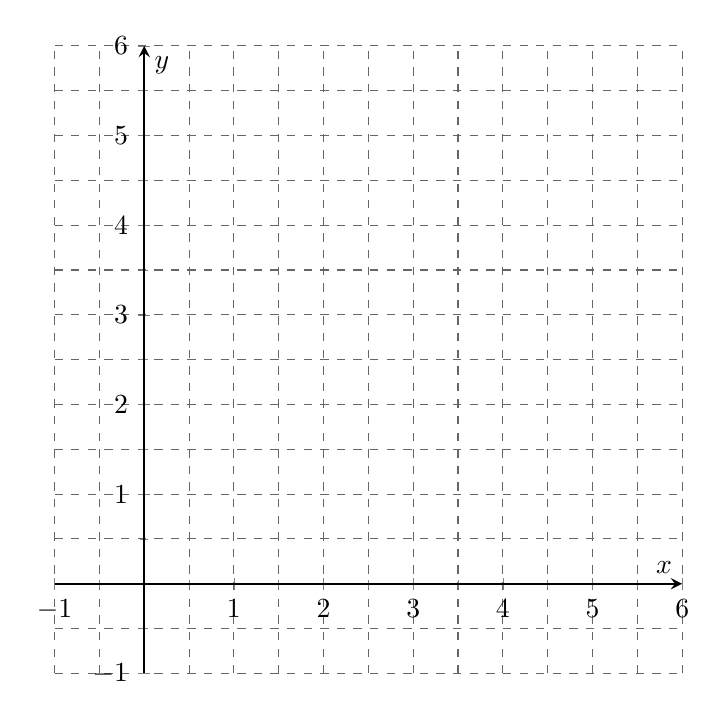
\begin{tikzpicture}
\begin{axis}[scale=1.4, thick, my style, xtick={-1,0,...,6}, ytick={-1,0,...,6},
xmin=-1, xmax=6, ymin=-1, ymax=6, minor y tick num=1,
        minor x tick num=1, mark size=3.0pt, grid=both, grid style={ thin, black!60, dashed}, axis equal image]
\end{axis}
\end{tikzpicture}




%\problem{5} Explain why $\displaystyle{\lim_{x \to 4}\frac{4-x}{|4-x|}}$ does not exist. 
%\vfill
%
%\problem{2} Evaluate $\displaystyle{\lim_{x \to 10}\frac{1}{(10-x)^2}}$ and justify your answer.
%\vfill
\end{document}